\documentclass{article}
\usepackage{iclr2027_conference,times}
\usepackage{amsmath,amssymb,booktabs,array,microtype,graphicx}
\usepackage{hyperref,url}
\usepackage{tikz}
\usetikzlibrary{arrows.meta}
\hypersetup{hidelinks}
\title{Forecast-Aware Imputation Portfolios:\\Objective Alignment and Transfer}
\author{Anonymous Authors}

\begin{document}
\maketitle

\begin{abstract}
Choosing how to complete a missing history changes the input to a frozen time-series forecaster. A useful selection rule must improve downstream prediction under the information available at deployment. We compare source-trained forecast portfolios using complete-history teacher supervision, matched aggregation objectives, and fixed combinations of the same candidate predictions. A small shared gate trained on the error of its returned forecast improves on a matched member-error objective during source development. A subsequent frozen confirmation on four new source families does not preserve that ordering. At horizon 96, the primary gate reduces MSE relative to a seven-candidate median by 5.90\% for Chronos-2 and 4.72\% for TimesFM 2.5, while MAE changes by $-1.02\%$ and $+0.80\%$, respectively. It also fails to improve on source-fixed convex combinations. Original missing histories show no consistent advantage. A separate three-forecaster budget study finds that the same change in imputer training can have opposite downstream effects. These results distinguish objective alignment during source fitting from reliable transfer of an imputation portfolio, and identify static aggregation and available historical information as necessary comparison conditions.
\end{abstract}

\section{Introduction}

A frozen time-series forecaster receives the history supplied by a data-processing procedure. Missing observations introduce several choices: complete the history with one imputer, use the forecaster's supported missing-input interface, or combine forecasts obtained from multiple completions. Each choice can preserve the same observed values and still produce a different future prediction. Selection must therefore be evaluated through the resulting forecast, with common information boundaries and a common outcome scale.

An objective that accurately describes the returned forecast can improve source fitting without producing a better transferable rule. In our source-development experiment, training the same small TimesFM portfolio gate on the error of its weighted prediction gives MSE 1.492189, compared with 1.499097 for a weighted member-error objective. After freezing both gates and evaluating new sources, the ordering reverses: the corresponding MSEs are 1.158096 and 1.132753. The candidate pool, representations and fitting budgets are matched within each comparison. This example motivates examining objective choice together with transfer and strong fixed combinations.

The distinction between imputation accuracy and prediction accuracy is established in missing-data research~\citep{lemorvan2021good}. Downstream evaluation is included in TSI-Bench, CleanIMP and ImputeGAP~\citep{du2024tsibench,cleanimp,nater2025imputegap}. Forecasting-oriented pairwise imputation selection and aggregation also have precedents~\citep{utama2026duel}, and forecast portfolios can be fitted using historical validation windows~\citep{kayaalp2025chroma}. The question studied here is narrower: whether source supervision for a fixed forecaster's imputation portfolio yields reliable improvements over aggregation using the same candidate forecasts.

Two difficulties affect this comparison. First, individual candidate costs do not describe the cost of their returned combination: aggregation changes the decision being optimized. Second, source-generated supervision may order candidates differently from the actual future in a new setting. Matching the learner across objectives addresses the first comparison, while freezing it before evaluating new sources addresses the second. Native missing-input semantics, target-prefix fitting, and originally unobserved future labels must be held explicit in both stages.

We study a shared gate that combines seven forecasts from six imputers and a native-input procedure. The complete-history prediction of the same frozen backbone supplies source supervision. Matched controls change the aggregation objective or replace this teacher with actual source future labels. We evaluate both MAE and MSE after training-prefix standardization, preserve the original future observation mask, and retain fixed convex combinations and forecast medians as strong controls. The empirical contribution is the resulting separation of source objective effects, confirmation behavior, and imputer-budget effects. The evidence supports conditional comparisons among these procedures; it does not establish a generally superior learned selector.

\section{Prediction Task and Comparison Conditions}
\label{sec:setting}

An observed context has length $L$ and $D$ variables, with unavailable values represented by an observation mask. A finite imputer preserves every observed entry. The evaluated finite procedures are LOCF, linear interpolation, seasonal lag, multivariate nearest neighbors, SAITS and TimeMixer++. The last two fit historical target-data prefixes; their backbones are not retrained jointly with the forecaster. The seventh candidate uses the forecasting model's missing-input behavior with an explicit empty-input fallback. MoTM supplies an additional pretrained imputation reference~\citep{motmsoftware}. Chronos-2 receives a joint multivariate context, whereas TimesFM 2.5 is invoked separately for each target~\citep{ansari2025chronos2,google2025timesfm25}.

Let $Y\in\mathbb R^{H\times K}$ denote the future, $V$ its original observation mask, and $P$ a point prediction. With target scale $s_k$ fitted from the observed training prefix and $n_k=\sum_hV_{hk}$, the principal errors are
\begin{align}
 \operatorname{MAE}(P,Y)&=\frac1K\sum_{k=1}^{K}\frac1{n_k}\sum_{h:V_{hk}=1}\frac{|P_{hk}-Y_{hk}|}{s_k},\\
 \operatorname{MSE}(P,Y)&=\frac1K\sum_{k=1}^{K}\frac1{n_k}\sum_{h:V_{hk}=1}\frac{(P_{hk}-Y_{hk})^2}{s_k^2}.
\end{align}
Unknown future entries are not filled to create scoring labels. Raw-scale errors and imputation reconstruction errors are auxiliary. All compared procedures share the evaluation contexts and prefix statistics. A procedure that queries multiple candidate histories must account for all corresponding forecasting work; the small size of a gate does not remove that cost.

\section{Forecast-Risk Supervision for Imputation Portfolios}
\label{sec:forecast_gate}

\paragraph{Candidate forecasts.}
Let $O\in(\mathbb{R}\cup\{\mathrm{NaN}\})^{L\times D}$ denote an observed multivariate history and let $F_H$ denote the fixed point-forecasting interface at horizon $H$. Six imputation procedures produce completed histories $C_a=I_a(O)$, preserving every observed entry. A seventh procedure uses the predictor's supported missing-input interface. Its empty-input fallback uses LOCF and historical-prefix medians: Chronos applies a shared fallback when any input channel is empty, whereas TimesFM applies the fallback to each empty target separately. The resulting forecasts are $P_a=F_H(C_a)$ for $a\in\{1,\ldots,7\}$, with the seventh argument interpreted according to this missing-input procedure. Both forecasting backbones retain their original parameters.

For target $k$, let $\mu_k$ and $s_k$ be the mean and population standard deviation of its observed historical fitting prefix. At least two observations are required; a standard deviation at most $10^{-12}$ is replaced by one and recorded. These statistics define $Z_{a,hk}=(P_{a,hk}-\mu_k)/s_k$. Forecasting inputs retain their original scale. Chronos uses one portfolio decision for both evaluated targets, so $z_a=\operatorname{vec}(Z_a)\in\mathbb{R}^{2H}$. TimesFM uses separate decisions, each with $z_a\in\mathbb{R}^{H}$. Write $q$ for the dimension of the applicable forecast vector.

\paragraph{Available representation and shared gate.}
Each candidate has 33 observable features: 21 summaries of the observed history and its completion, and 12 summaries of its queried forecast. Forecast summaries describe changes from LOCF, distance from the median of the six finite-imputation forecasts, temporal variation, and departure from the last LOCF history value. The two quantile-related fields remain zero in this point-forecast evaluation. Dataset identifiers, artificial-mask labels, actual future values, and artificially hidden historical values are excluded from the gate input.

A shared linear layer with 16 ReLU units maps each candidate feature vector $x_a$ to $h_a$. The mean $\bar h=7^{-1}\sum_a h_a$ represents the candidate set. A second 16-unit ReLU layer and a scalar output layer score $[h_a;\bar h]$, with an additional learned bias for each candidate. Softmax converts the seven scores into weights $w_\theta(x)\in\Delta_7$, where $\Delta_7=\{w\geq0:\sum_a w_a=1\}$. Feature centering and scaling use source training rows only, with the source family weights; scales have a floor of $10^{-6}$, and standardized features are clipped to $[-10,10]$. Each gate has 1,096 trainable parameters. The prediction averages the weight vectors from the three prespecified seeds and returns
\begin{equation}
 \widehat z=\sum_{a=1}^{7}\bar w_a z_a,
 \qquad \bar w_a=\frac{1}{3}\sum_{j=1}^{3}w_{\theta_j,a}.
 \label{eq:gate_prediction}
\end{equation}
The deployed gate ensemble therefore has 3,288 trainable parameters per backbone. Each TimesFM target receives its own weights; Chronos shares weights across its two targets. Equation~\ref{eq:gate_prediction} combines predictions and does not define a unique completed input history.

\paragraph{Supervision from complete source histories.}
For a source history $X$ whose values are available before artificial masking, the same frozen forecaster provides a teacher vector $t$ from $F_H(X)$, standardized by the same prefix statistics. Only source training histories supply this supervision. The teacher does not require the actual future associated with that source history, and its complete-history input is unavailable to the deployed gate. The teacher is the backbone's selected point output; no assumption that it equals the true conditional future mean is imposed by the implementation.

The primary objective evaluates the forecast actually returned by the gate:
\begin{equation}
 \mathcal{L}_{\mathrm{ens}}(w)
 =\frac{1}{q}\left\|\sum_a w_a z_a-t\right\|_2^2.
 \label{eq:gate_teacher_loss}
\end{equation}
The matched control instead minimizes
$\mathcal{L}_{\mathrm{mem}}(w)=q^{-1}\sum_a w_a\|z_a-t\|_2^2$
with the same representation, architecture, training histories and optimization budget. For nonnegative weights summing to one, their difference is the established ensemble-dispersion identity~\citep{krogh1994ensembles}:
\begin{equation}
 \mathcal{L}_{\mathrm{mem}}(w)-\mathcal{L}_{\mathrm{ens}}(w)
 =\frac{1}{q}\sum_a w_a\left\|z_a-\sum_b w_bz_b\right\|_2^2.
 \label{eq:gate_dispersion}
\end{equation}
This identity motivates a matched objective comparison for weighted means. It neither applies directly to median aggregation nor guarantees improved prediction of the real future.

\paragraph{Cached quadratic objective.}
Let $b=\operatorname{median}_a z_a$, $d_a=z_a-b$, and $G_{ab}=q^{-1}d_a^\top d_b$. The stored single-candidate teacher risks are measured relative to the same reference:
$r_a=q^{-1}(\|z_a-t\|_2^2-\|b-t\|_2^2)$.
Setting $c_a=(G_{aa}-r_a)/2$ gives
\begin{equation}
 \mathcal{L}_{\mathrm{ens}}(w)-q^{-1}\|b-t\|_2^2
 =w^\top G w-2c^\top w,
 \qquad
 \mathcal{L}_{\mathrm{mem}}(w)-q^{-1}\|b-t\|_2^2=w^\top r.
 \label{eq:gate_quadratic}
\end{equation}
The omitted term is independent of the gate parameters. Training therefore reuses the candidate forecasts and teacher-risk records and differentiates only through the small gate. A source-fixed convex combination minimizes the family-weighted quadratic objective over $\Delta_7$; a source-fixed single minimizes the corresponding individual teacher risk. A further matched control replaces $t$ with the actual standardized source future while retaining the same gate and fitting budget.

\paragraph{Fitting and evaluation boundary.}
Source development leaves one family out at a time and fits on the earlier source training histories of the remaining families. Final source models use the original 165 training origins from 15 families, with 5,940 artificial-mask episodes. The optimization schedule is fixed at 25 epochs, batch size 128, AdamW learning rate $10^{-3}$, weight decay $10^{-3}$ and gradient-norm limit one. The three seeds are 5101, 5102 and 5103. Validation outcomes do not select epochs or seeds. All final source parameters are fixed before new confirmation data are evaluated.

The primary confirmation uses $L=H=96$. The same source models are applied at $H=192$ without retraining, providing a separate horizon-transfer evaluation. Both MAE and MSE are computed on originally observed future target entries after training-prefix standardization. An input must have at least 48 observed future entries per target at $H=96$ and at least 96 at $H=192$. The predictor must evaluate up to seven distinct candidate histories before gate application; batching and reuse of identical effective inputs reduce calls but do not turn this procedure into prediction-free imputation selection. The MoTM comparator and eight-member forecast median have a separately recorded additional-candidate budget.


\begin{figure}[t]
\centering
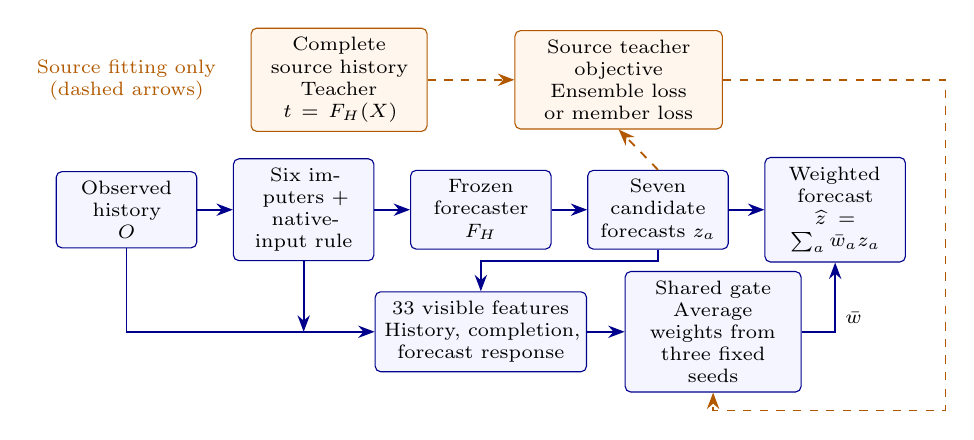
\begin{tikzpicture}[
  x=1cm,y=1cm,>=Stealth,
  box/.style={draw=blue!55!black,rounded corners=2pt,fill=blue!4,align=center,minimum height=.75cm,text width=1.55cm,font=\scriptsize},
  training/.style={draw=orange!70!black,fill=orange!7,rounded corners=2pt,align=center,minimum height=.62cm,text width=2.0cm,font=\scriptsize},
  flow/.style={->,line width=.65pt,draw=blue!55!black},
  supervision/.style={->,dashed,line width=.65pt,draw=orange!70!black}
]
\node[box] (observed) at (0,0) {Observed history\\$O$};
\node[box] (candidates) at (2.25,0) {Six imputers +\\native-input rule};
\node[box] (forecaster) at (4.5,0) {Frozen forecaster\\$F_H$};
\node[box] (points) at (6.75,0) {Seven candidate\\forecasts $z_a$};
\node[box] (output) at (9.0,0) {Weighted forecast\\$\widehat z=\sum_a\bar w_a z_a$};
\draw[flow] (observed) -- (candidates);
\draw[flow] (candidates) -- (forecaster);
\draw[flow] (forecaster) -- (points);
\draw[flow] (points) -- (output);
\node[box,text width=2.45cm] (features) at (4.5,-1.55) {33 visible features\\History, completion,\\forecast response};
\node[box,text width=2.0cm] (gate) at (7.45,-1.55) {Shared gate\\Average weights from\\three fixed seeds};
\draw[flow] (points.south) -- (6.75,-.65) -- (4.5,-.65) -- (features.north);
\draw[flow] (observed.south) -- (0,-1.55) -- (features.west);
\draw[flow] (candidates.south) -- (2.25,-1.55);
\draw[flow] (features) -- (gate);
\draw[flow] (gate.east) -| node[pos=.6,right,font=\scriptsize] {$\bar w$} (output.south);
\node[training] (teacher) at (2.7,1.65) {Complete source history\\Teacher $t=F_H(X)$};
\node[training,text width=2.4cm] (loss) at (6.25,1.65) {Source teacher objective\\Ensemble loss or member loss};
\draw[supervision] (teacher) -- (loss);
\draw[supervision] (points.north) -- (loss.south);
\draw[supervision] (loss.east) -- (10.4,1.65) -- (10.4,-2.55) -- (7.45,-2.55) -- (gate.south);
\node[font=\scriptsize,orange!70!black,align=center] at (0,1.65) {Source fitting only\\(dashed arrows)};
\end{tikzpicture}

\caption{The shared imputation portfolio. Solid arrows show prediction-time computation; dashed arrows show source teacher supervision of the gate. The feature block uses observed history, candidate completions and queried forecasts. The forecaster remains frozen. Deployment does not receive the complete source history or its teacher output, and the returned combination is a forecast rather than a unique completed history.}
\label{fig:r6_portfolio}
\end{figure}

\section{Source Development and Earlier Confirmation}
\label{sec:development}

The source population contains 15 data families with one evaluated multivariate item per dataset. It provides 165 training origins and 52 later validation origins, corresponding to 5,940 training and 1,872 validation masking tasks. Each origin contributes six masking mechanisms, three rates and two seeds. Source training futures end before the 60\% temporal boundary; validation contexts follow that boundary. Imputers use historical prefixes, and held-family selector fits exclude that family's training origins. Multiple masks of one history remain in the same group. Appendix~\ref{app:source} reports the actual source coverage and fitting settings.

Table~\ref{tab:r6_source} compares the two teacher objectives using the same shared network and three fixed seeds. Direct ensemble-error training improves both mean metrics for both forecasters relative to member-error training. Its improvement over the seven-candidate median is small for Chronos: 0.20\% in MAE and 0.97\% in MSE, with five joint family wins and eight joint losses. TimesFM improves by 2.37\% and 4.07\%, with eleven joint family wins and four joint losses. Family heterogeneity therefore matters even before independent confirmation.

\begin{table}[t]
\caption{Held-family source development at $L=H=96$. Equal-family standardized MAE/MSE are shown. Both gates have the same architecture, representation and fitting schedule.}
\label{tab:r6_source}
\centering\small
\begin{tabular}{lrrrr}
\toprule
 & \multicolumn{2}{c}{Chronos-2} & \multicolumn{2}{c}{TimesFM 2.5}\\
Procedure & MAE & MSE & MAE & MSE\\
\midrule
Ensemble teacher loss & .779079 & 1.543561 & .754242 & 1.492189\\
Member teacher loss & .795789 & 1.639266 & .758550 & 1.499097\\
Source-fixed convex mixture & .780687 & 1.555598 & .771366 & 1.529399\\
Seven-candidate median & .780606 & 1.558757 & .772570 & 1.555558\\
\bottomrule
\end{tabular}
\end{table}

The gate study followed earlier source-trained ranking experiments. A cost-sensitive pairwise ranker, using the established portfolio-selection construction~\citep{xu2012evaluating}, selected three candidate forecasts. Its frozen confirmation on 373 windows from nine new families did not reproduce its development advantage, including 164 histories with original missingness. A later matched comparison over 35 candidate triples improved development results but failed to transfer consistently in an 823-task follow-up: gains on new synthetic histories occurred for Chronos and reversed for TimesFM. These outcomes remain part of the evidence. Subsequent gate evaluation on that already-used follow-up data is a development diagnostic, not a fresh confirmation. The gate was then fixed for the four-source confirmation described below.

Appendix~\ref{app:source-controls} reports subsequent matched source-supervision and original-missing source-extension checks, retaining their retrospective development status.

\section{Independent Confirmation Protocol}
\label{sec:r6_protocol}

\paragraph{Data sources and chronology.}
The final source gates were fixed before constructing a new confirmation cohort. The cohort uses Beijing Multi-Site Air Quality, Appliances Energy Prediction, hourly Bike Sharing, and the environmental measurements from Occupancy Detection~\citep{uci2017beijing,uci2017appliances,uci2013bike,uci2016occupancy}. These sources were outside the selector's training and earlier evaluation catalogs. This separation concerns selector development; it does not establish that the released forecasting models never encountered these sources during pretraining. Source files, preprocessing, target choices and task identities were recorded before forecasting errors were examined.

Table~\ref{tab:r6_coverage} reports the retained input population. Each input is evaluated at both $H=96$ and $H=192$, with $L=96$. The cohort contains 381 distinct history origins and 1,522 input tasks. Of these, 1,152 are artificial-mask tasks from 32 complete histories, with 36 masking conditions per history. The remaining 370 inputs retain their original observations. Horizons, masks and panels can share a history origin and are not independent samples.

\begin{table}[t]
\caption{New confirmation coverage. Input tasks are shared between the two prediction horizons. The 12 Beijing stations form one source family.}
\label{tab:r6_coverage}
\centering\small
\begin{tabular}{lrrrr}
\toprule
Source & Items & Variables & Origins & Input tasks \\
\midrule
Beijing Multi-Site & 12 & 11 & 320 & 608 \\
Appliances & 1 & 26 & 20 & 304 \\
Bike Sharing & 1 & 6 & 22 & 306 \\
Occupancy measurements & 1 & 4 & 19 & 304 \\
\midrule
Total & 15 & -- & 381 & 1,522 \\
\bottomrule
\end{tabular}
\end{table}

\paragraph{Targets and observation semantics.}
The two targets are PM2.5/PM10 for Beijing, appliance/lighting energy for Appliances, casual/registered rental counts for Bike Sharing, and temperature/humidity for Occupancy. Identifiers and categorical calendar fields are excluded. The random variables supplied with Appliances, the bike-count total derived from its two targets, and the occupancy classification label and target-derived humidity ratio are also excluded. The remaining input variables retain the provider's numerical representation. The Appliances release includes interpolated airport-weather covariates, while its energy targets are measured at ten-minute resolution.

Beijing measurements use an hourly grid and preserve their original NA entries. Bike Sharing supplies 17,379 hourly records; its nominal hourly grid has 17,544 positions, with 165 unrecorded hours retained as unknown. The three Occupancy files are merged chronologically. Timestamp rounding changes no time by more than one second; 20,560 records map to a 22,741-minute grid with 2,181 unrecorded minutes and no duplicate rounded rows. Unknown time-bin values are never replaced by zero or treated as future truth. Their reporting or clock-related causes are not identified. Consequently, original-NA histories, nominal time-grid gaps and complete-release controls are reported separately.

\paragraph{Eligibility and missingness.}
Imputer fitting and scoring statistics use the first 20\% of each item, requiring at least two observations in every retained channel. Origins follow the 60\% time boundary and the prescribed separation from prefix fitting. A stride of 288 separates a 96-step context and its maximum 192-step future. Eligibility requires at least 48 observed future values per target through step 96 and at least 96 through step 192. Up to 16 missing-context and 16 complete-context origins are retained per item by evenly spaced chronological selection. These strata do not estimate the population frequency of missingness.

Artificial masking uses complete observed histories and complete two-target futures through step 192. Up to eight origins per item are selected before masking. For Beijing this panel uses the first four station names in lexical order: their eligible-history counts are 1, 4, 0 and 3, and no replacement station is introduced. The other three sources contribute eight histories each. Six missingness mechanisms, rates 0.1/0.3/0.5 and seeds 8101/8102 define the 36 conditions per history. Whole-trajectory masks use prefix-only calibration; the same realized context is reused at both horizons. Original observation masks remain distinct from artificial masks. Exact comparisons of 96-step target histories and their first 96 future steps against 853 previously used windows found no duplicate window.

\paragraph{Models and comparison conditions.}
The two primary forecasters are the fixed Chronos-2 and TimesFM 2.5 revisions used in source development. Imputation uses the same six procedures, including SAITS and TimeMixer++ fitted for ten epochs on at most 64 prefix windows. MoTM uses its pinned released networks and unchanged observed-context adaptation. The confirmation retains 23 outputs: seven single-candidate forecasts, standalone MoTM, five forecast-aggregation controls, three small gates with different source supervision, their source-fixed convex/single controls, and the previous learned and fixed three-candidate procedures. The primary gate uses complete-history teacher supervision; the matched small-network controls change the aggregation loss or replace the teacher with actual source future labels. All source models are fixed before confirmation.

The native forecasting interfaces were checked at both horizons on finite and missing inputs from all four sources. All 32 comparisons agreed with direct vendor calls, and the forecasting parameters remained unchanged. Effective duplicate inputs can reuse predictions. The primary gate still requires up to seven candidate-history evaluations, while the eight-member MoTM median can require one additional candidate. Source fitting, input completion, forecasting and gate execution have separate costs.

\paragraph{Metrics and interpretation.}
MAE and MSE are computed after standardization by observed-prefix statistics and only at originally observed future entries. Targets are averaged within a task, masks within an origin, origins within an item, items within a dataset, and datasets within a source family. Each horizon and observation panel is reported separately. Paired source differences and joint MAE/MSE win/loss counts accompany aggregate effects. Source-resampling ranges describe sensitivity to reweighting the observed sources; four purposively selected source families do not establish a broad population significance claim. The original-NA panel has one source family, and its station count is not substituted for the number of families.


\paragraph{Candidate evaluation budget.}
On the synthetic confirmation panel, the seven-candidate bank contains an average of 6.332 distinct effective contexts per Chronos input and 5.989 per TimesFM input, after reuse of identical effective inputs. Adding MoTM raises these averages to 7.242 and 6.832. The maxima are seven and eight, respectively. These counts describe candidate-context evaluations in the recorded implementation, not backend invocation counts, FLOPs or latency. Imputer fitting and completion add separate costs. A static combination with zero weights could omit candidates in a dedicated implementation; sharing the full bank here does not imply equal minimum deployment cost for every policy.

\section{Confirmation Results and Transfer Limits}
\label{sec:r6_results}

\paragraph{Main synthetic-missingness comparison.}
Table~\ref{tab:r6_main} reports the prespecified $H=96$ comparison across the four new source families. Relative to the seven-candidate median, the primary ensemble-loss gate changes Chronos-2 MAE/MSE by $-1.02\%/-5.90\%$ and TimesFM~2.5 by $+0.80\%/-4.72\%$. Both MSEs decrease, while the MAE effects differ. Relative to the median that additionally includes MoTM, the primary gate has higher MAE and lower MSE for both backbones. Its two errors are also slightly higher than those of the source-fixed convex mixture. The confirmation therefore does not support a consistent advantage for the adaptive ensemble-loss gate over the stronger static controls.

\begin{table}[t]
\caption{Frozen confirmation on artificially masked histories at $H=96$. Entries are training-prefix-standardized downstream MAE/MSE, averaged equally across four source families. The cohort has 32 original histories and 1,152 masking tasks. The MoTM median uses one additional candidate. Lower values are better.}
\label{tab:r6_main}
\centering\small
\begin{tabular}{lrrrr}
\toprule
 & \multicolumn{2}{c}{Chronos-2} & \multicolumn{2}{c}{TimesFM 2.5} \\
Procedure & MAE & MSE & MAE & MSE \\
\midrule
Ensemble teacher loss (primary) & .608321 & 1.110985 & .624733 & 1.158096 \\
Member teacher loss & .593649 & 1.134564 & .605122 & 1.132753 \\
Source future supervision & .616020 & 1.147136 & .600364 & 1.130239 \\
Source-fixed convex mixture & .600751 & 1.109923 & .616414 & 1.148950 \\
Seven-candidate median & .614601 & 1.180633 & .619774 & 1.215528 \\
Median including MoTM & .605507 & 1.139357 & .611607 & 1.171881 \\
\bottomrule
\end{tabular}
\end{table}

\paragraph{Matched objectives do not preserve their development ordering.}
For Chronos-2, the member-loss control has lower MAE and higher MSE than the primary gate. For TimesFM, it improves both metrics. The primary TimesFM gate achieves no joint MAE/MSE family win against the member-loss control and incurs three joint losses. Replacing the complete-history teacher with actual source future supervision also improves both aggregate TimesFM errors. Chronos shows the opposite aggregate ordering for this supervision comparison, but its primary gate wins jointly on only one family and loses jointly on three. This concentration of the aggregate benefit prevents a source-independent interpretation of teacher superiority.

\paragraph{Original missingness.}
The Beijing subset with originally incomplete histories contains 192 origins from 12 stations within one source family. The primary Chronos gate obtains MAE/MSE of .955657/1.950378, compared with .951353/1.941988 for guarded native input. The corresponding TimesFM values are .982291/2.050711 and .971437/2.021100. Neither backbone gains from the primary gate in this comparison. Appendix~\ref{app:r6_full} retains the classical, fixed-mixture and median controls as well. The 128 complete-history controls return identical predictions across the imputation-preserving mixture procedures and are reported separately. Gaps introduced by nominal time-grid reconstruction remain a separate observation category.

\paragraph{Scope of the evidence.}
The primary method was fixed before the new cohort's outcomes were examined. All 23 procedures, both horizons and the registered observation panels are retained. Independent reconstruction checks cover 140,024 method forecast vectors and 27,396 gate decisions; prediction reconstruction differences are zero, and metric recomputation differs by at most $3.49\times10^{-10}$, including raw-scale metrics. These checks establish computational consistency. Four purposively selected source families, shared histories across masks and horizons, and a single source family with original missingness limit broader conclusions. Subsequent analysis of this cohort is developmental reuse and cannot replace its original confirmation result.


\section{Imputer Training Budget and Predictor Dependence}
\label{sec:budget}

A separate development sensitivity study evaluates ETTh1, current-velocity and electricity data. Each contributes four registered validation histories under six masking conditions. SAITS and TimeMixer++ retain their architecture and initialization under budgets of 10 epochs/64 masked windows, 50 epochs/64 windows and 50 epochs/512 windows. The larger batch includes the original windows, with all additional data taken from the same fitting prefixes. This produces 18 fitted imputers. One history per dataset was examined first; three further histories were evaluated with the settings and fitted models fixed. TiRex provides a third frozen forecaster for this study~\citep{auer2025tirex}.

\begin{table}[t]
\caption{TimeMixer++ on four current-velocity histories. Six masks are averaged within a history and then histories are equally weighted. The same larger imputation budget has different downstream effects across forecasters.}
\label{tab:budget-origins}
\centering\small
\begin{tabular}{lrrrr}
\toprule
 & \multicolumn{2}{c}{10 epochs / 64 windows} & \multicolumn{2}{c}{50 epochs / 512 windows}\\
Forecaster & MAE & MSE & MAE & MSE\\
\midrule
Chronos-2 & .737114 & .827770 & .763693 & .872270\\
TimesFM 2.5 & .669345 & .683377 & .657149 & .664951\\
TiRex & .616648 & .620702 & .626207 & .635902\\
\bottomrule
\end{tabular}
\end{table}

Table~\ref{tab:budget-origins} shows opposite responses to a common change in imputation budget. Both metrics improve on three of four TimesFM histories, zero Chronos histories and one TiRex history. The two independent-target forecasters also disagree, so joint versus independent input handling alone does not explain this comparison. Across the three datasets, the 50/512 seven-candidate forecast median improves both mean metrics on ETTh1 and worsens both on current velocity and electricity for all three forecasters. The direction is not universal at the individual-history level.

Increasing the budget can also yield nonmonotonic effects. For the initial electricity SAITS history under Chronos, MAE/MSE changes from .544629/.678087 at 10/64 to .418077/.466078 at 50/64, then to .647737/.911696 at 50/512. Separate crossed replacements of target and other input columns expose interactions in joint-context forecasts. These are controlled observations within fixed architectures and fitting prefixes. They do not estimate fully tuned imputer capacity or establish a general ranking of imputation algorithms.

\section{Related Work and Limitations}

\paragraph{Missing-data prediction and aggregation.}
\citet{lemorvan2021good} study imputation followed by prediction, including consequences of retaining a complete-data regression function. Our experiment holds a pretrained vector-output forecaster fixed while changing its input completion or combining candidate forecasts. Complete-history supervision relates to distillation~\citep{menon2021statistical}, and the member-versus-ensemble squared-loss identity is established~\citep{krogh1994ensembles}. These ingredients motivate matched controls; they do not supply a new general theorem or a transfer guarantee.

\paragraph{Evaluation and portfolio selection.}
TSI-Bench, CleanIMP and ImputeGAP include downstream evaluation of imputation~\citep{du2024tsibench,cleanimp,nater2025imputegap}. Pairwise forecasting-oriented imputation comparison and top-three aggregation are studied by \citet{utama2026duel}. Chroma fits pretrained forecasting portfolios using historical validation~\citep{kayaalp2025chroma}. Learning how weights vary across series, forecast positions and quantiles also has established precedents~\citep{hasson2023ensembling}. SwiftTS estimates pretrained models' post-fine-tuning performance for model selection~\citep{zhang2025swiftts}. Our comparisons instead hold the forecaster fixed and vary its input completion or combine the resulting forecasts. Neither forecast aggregation nor position-dependent combination is claimed as a new construction. Static combinations and historical information remain essential controls.

\paragraph{Scope.}
Confirmation covers two backbones, two horizons and four purposively selected source families; only one contributes original-NA histories. Repeated masks do not enlarge the 165-history source-training population. Source and confirmation conditions differ along several dimensions, preventing attribution to one failure mechanism. Missing future labels restrict scoring to observed outcomes, and forecaster pretraining exclusion is not established for every source. The budget study covers three forecasters but only three datasets and 12 histories. These conditional comparisons do not establish that learned selection cannot succeed.

\section{Conclusion}

Forecast-aware imputation portfolios must be assessed through downstream prediction under explicit deployment information. Matching the objective to the returned forecast improves the studied source-development gates, but the frozen confirmation does not establish a consistent advantage over fixed convex mixtures and strong forecast medians. Original missingness and a separate imputer-budget study further expose conditional behavior across forecasting models. Reliable evidence for learned imputation selection therefore requires strong fixed combinations, distinct source and confirmation stages, both MAE and MSE, and clear accounting of available history and forecasting cost.

\bibliography{tsfm_fais_iclr2027,tsfm_fais_r5_draft,tsfm_fais_r6_additions}
\bibliographystyle{iclr2027_conference}

\clearpage
\appendix
\section{Complete Confirmation Comparisons}
\label{app:r6_full}
Tables~\ref{tab:r6_all_synthetic_h96}--\ref{tab:r6_all_native_h192} retain all 23 frozen procedures on the synthetic and originally missing panels at both horizons. The two targets are averaged within an input, followed by equal weighting of histories, items, datasets and source families. Bold identifies the lowest displayed score within each column. Shared histories across masks and horizons are not independent samples.
\begin{table}[!htbp]
\caption{Artificial missingness: 32 complete histories, 1,152 masking inputs and four source families. Horizon 96. Standardized downstream MAE/MSE; lower is better.}
\label{tab:r6_all_synthetic_h96}
\centering\small
\begin{tabular}{lrrrr}
\toprule
 & \multicolumn{2}{c}{Chronos-2} & \multicolumn{2}{c}{TimesFM 2.5}\\
Procedure & MAE & MSE & MAE & MSE\\
\midrule
LOCF & 0.664132 & 1.477673 & 0.673797 & 1.507488\\
Linear interpolation & 0.679381 & 1.572613 & 0.683644 & 1.590224\\
Seasonal lag & 0.631647 & 1.223257 & 0.623139 & 1.196848\\
Multivariate nearest neighbors & 0.659391 & 1.294877 & 0.663057 & 1.349377\\
SAITS & 0.650770 & 1.270880 & 0.650017 & 1.292376\\
TimeMixer++ & 0.671324 & 1.296532 & 0.669241 & 1.310951\\
Guarded native input & 0.604171 & 1.200309 & 0.672877 & 1.539210\\
MoTM & 0.635111 & 1.222468 & 0.638219 & 1.263218\\
Mean of six finite candidates & 0.628933 & 1.173273 & 0.628167 & 1.180577\\
Median of six finite candidates & 0.624324 & 1.205464 & 0.621990 & 1.212519\\
Mean of seven candidates & 0.620103 & 1.144141 & 0.630054 & 1.194909\\
Median of seven candidates & 0.614601 & 1.180633 & 0.619774 & 1.215528\\
Median including MoTM & 0.605507 & 1.139357 & 0.611607 & 1.171881\\
Individual teacher ranking, top three & 0.587200 & 1.104139 & 0.605561 & 1.175001\\
Source-fixed individual-risk triple & 0.594789 & 1.148699 & 0.625741 & 1.242735\\
Learned triple: combination teacher risk & 0.586873 & 1.085500 & 0.608002 & 1.177663\\
Learned triple: member teacher risk & \textbf{0.581795} & \textbf{1.085192} & 0.615569 & 1.216673\\
Source-fixed combination-risk triple & 0.594789 & 1.148699 & 0.619040 & 1.207129\\
Ensemble teacher gate (primary) & 0.608321 & 1.110985 & 0.624733 & 1.158096\\
Member teacher gate & 0.593649 & 1.134564 & 0.605122 & 1.132753\\
Source future-supervised gate & 0.616020 & 1.147136 & \textbf{0.600364} & \textbf{1.130239}\\
Source-fixed convex mixture & 0.600751 & 1.109923 & 0.616414 & 1.148950\\
Source-fixed single candidate & 0.604171 & 1.200309 & 0.623139 & 1.196848\\
\bottomrule
\end{tabular}
\end{table}

\begin{table}[!htbp]
\caption{Artificial missingness: 32 complete histories, 1,152 masking inputs and four source families. Horizon 192. Standardized downstream MAE/MSE; lower is better.}
\label{tab:r6_all_synthetic_h192}
\centering\small
\begin{tabular}{lrrrr}
\toprule
 & \multicolumn{2}{c}{Chronos-2} & \multicolumn{2}{c}{TimesFM 2.5}\\
Procedure & MAE & MSE & MAE & MSE\\
\midrule
LOCF & 0.700649 & 1.554350 & 0.715843 & 1.601017\\
Linear interpolation & 0.709172 & 1.615842 & 0.725900 & 1.694804\\
Seasonal lag & 0.665305 & 1.314595 & 0.666854 & 1.316702\\
Multivariate nearest neighbors & 0.688642 & 1.376007 & 0.707498 & 1.485056\\
SAITS & 0.688555 & 1.380330 & 0.698676 & 1.444043\\
TimeMixer++ & 0.705086 & 1.392193 & 0.715922 & 1.454231\\
Guarded native input & 0.633150 & 1.255335 & 0.713977 & 1.638922\\
MoTM & 0.667095 & 1.303082 & 0.683597 & 1.381504\\
Mean of six finite candidates & 0.663127 & 1.260948 & 0.672728 & 1.306693\\
Median of six finite candidates & 0.658360 & 1.294804 & 0.667433 & 1.341754\\
Mean of seven candidates & 0.653054 & 1.227724 & 0.674032 & 1.317249\\
Median of seven candidates & 0.646870 & 1.264564 & 0.664383 & 1.338877\\
Median including MoTM & 0.637855 & 1.222324 & 0.655845 & 1.293378\\
Individual teacher ranking, top three & 0.622052 & 1.189024 & 0.650046 & 1.292228\\
Source-fixed individual-risk triple & 0.624603 & 1.215744 & 0.668339 & 1.358296\\
Learned triple: combination teacher risk & \textbf{0.617015} & \textbf{1.157891} & 0.653202 & 1.298539\\
Learned triple: member teacher risk & 0.618107 & 1.176196 & 0.659582 & 1.334614\\
Source-fixed combination-risk triple & 0.624603 & 1.215744 & 0.662784 & 1.329668\\
Ensemble teacher gate (primary) & 0.636745 & 1.178526 & 0.664386 & 1.265550\\
Member teacher gate & 0.625210 & 1.197344 & 0.645186 & \textbf{1.240919}\\
Source future-supervised gate & 0.649898 & 1.239344 & \textbf{0.642417} & 1.245513\\
Source-fixed convex mixture & 0.630231 & 1.179018 & 0.659963 & 1.266592\\
Source-fixed single candidate & 0.633150 & 1.255335 & 0.666854 & 1.316702\\
\bottomrule
\end{tabular}
\end{table}

\begin{table}[!htbp]
\caption{Original missingness: 192 Beijing histories from 12 stations in one source family. Horizon 96. Standardized downstream MAE/MSE; lower is better.}
\label{tab:r6_all_native_h96}
\centering\small
\begin{tabular}{lrrrr}
\toprule
 & \multicolumn{2}{c}{Chronos-2} & \multicolumn{2}{c}{TimesFM 2.5}\\
Procedure & MAE & MSE & MAE & MSE\\
\midrule
LOCF & \textbf{0.950132} & 1.943627 & 0.971925 & 2.019353\\
Linear interpolation & 0.950227 & 1.944724 & \textbf{0.969275} & \textbf{2.015033}\\
Seasonal lag & 0.974885 & 2.010805 & 0.989865 & 2.090399\\
Multivariate nearest neighbors & 0.961376 & 1.969753 & 0.986390 & 2.078360\\
SAITS & 0.957647 & 1.957036 & 0.984749 & 2.073282\\
TimeMixer++ & 0.961594 & 1.962200 & 0.980503 & 2.051087\\
Guarded native input & 0.951353 & \textbf{1.941988} & 0.971437 & 2.021100\\
MoTM & 0.967316 & 1.993144 & 0.988743 & 2.073599\\
Mean of six finite candidates & 0.956681 & 1.952902 & 0.977016 & 2.038406\\
Median of six finite candidates & 0.957101 & 1.955445 & 0.980046 & 2.048878\\
Mean of seven candidates & 0.955058 & 1.948091 & 0.975680 & 2.033217\\
Median of seven candidates & 0.956488 & 1.953139 & 0.978526 & 2.041793\\
Median including MoTM & 0.957342 & 1.955942 & 0.979453 & 2.043289\\
Individual teacher ranking, top three & 0.957032 & 1.956728 & 0.977873 & 2.033044\\
Source-fixed individual-risk triple & 0.955994 & 1.946929 & 0.982924 & 2.062434\\
Learned triple: combination teacher risk & 0.958852 & 1.956421 & 0.980450 & 2.040928\\
Learned triple: member teacher risk & 0.955966 & 1.955191 & 0.979422 & 2.038913\\
Source-fixed combination-risk triple & 0.955994 & 1.946929 & 0.981958 & 2.056250\\
Ensemble teacher gate (primary) & 0.955657 & 1.950378 & 0.982291 & 2.050711\\
Member teacher gate & 0.952588 & 1.942716 & 0.979920 & 2.040645\\
Source future-supervised gate & 0.956171 & 1.953695 & 0.980731 & 2.047140\\
Source-fixed convex mixture & 0.954660 & 1.946952 & 0.979966 & 2.043733\\
Source-fixed single candidate & 0.951353 & \textbf{1.941988} & 0.989865 & 2.090399\\
\bottomrule
\end{tabular}
\end{table}

\begin{table}[!htbp]
\caption{Original missingness: 192 Beijing histories from 12 stations in one source family. Horizon 192. Standardized downstream MAE/MSE; lower is better.}
\label{tab:r6_all_native_h192}
\centering\small
\begin{tabular}{lrrrr}
\toprule
 & \multicolumn{2}{c}{Chronos-2} & \multicolumn{2}{c}{TimesFM 2.5}\\
Procedure & MAE & MSE & MAE & MSE\\
\midrule
LOCF & 1.003871 & 2.215710 & 1.033990 & 2.326283\\
Linear interpolation & 1.002549 & 2.215391 & 1.030748 & 2.318477\\
Seasonal lag & 1.008891 & 2.219830 & 1.038977 & 2.357782\\
Multivariate nearest neighbors & 1.004405 & 2.213127 & 1.040638 & 2.357744\\
SAITS & 1.002326 & 2.206226 & 1.038978 & 2.350760\\
TimeMixer++ & 1.003487 & 2.205822 & 1.033742 & 2.331863\\
Guarded native input & 0.999211 & 2.210220 & 1.032443 & 2.324450\\
MoTM & 1.010474 & 2.235865 & 1.040558 & 2.348499\\
Mean of six finite candidates & 1.000870 & 2.200697 & 1.031193 & 2.321433\\
Median of six finite candidates & 1.001998 & 2.206083 & 1.034343 & 2.330134\\
Mean of seven candidates & 0.999880 & 2.198561 & \textbf{1.030462} & 2.318470\\
Median of seven candidates & 1.001817 & 2.205530 & 1.033228 & 2.324191\\
Median including MoTM & 1.002224 & 2.206333 & 1.034025 & 2.325857\\
Individual teacher ranking, top three & 1.002582 & 2.209810 & 1.032216 & \textbf{2.315772}\\
Source-fixed individual-risk triple & 1.000222 & 2.197967 & 1.036182 & 2.341873\\
Learned triple: combination teacher risk & 1.001785 & 2.202354 & 1.034049 & 2.322201\\
Learned triple: member teacher risk & 1.001781 & 2.207453 & 1.033022 & 2.319224\\
Source-fixed combination-risk triple & 1.000222 & 2.197967 & 1.035738 & 2.336656\\
Ensemble teacher gate (primary) & 1.000238 & 2.202889 & 1.034761 & 2.327239\\
Member teacher gate & 0.998896 & 2.204126 & 1.033196 & 2.319714\\
Source future-supervised gate & 0.999885 & 2.201400 & 1.031819 & 2.321118\\
Source-fixed convex mixture & \textbf{0.998834} & \textbf{2.197785} & 1.031979 & 2.323520\\
Source-fixed single candidate & 0.999211 & 2.210220 & 1.038977 & 2.357782\\
\bottomrule
\end{tabular}
\end{table}



\clearpage
\section{Development Data Coverage and Imputer Settings}
\label{app:source}

Table~\ref{tab:source-inventory} gives the actual evaluated source population. Each dataset contributes one evaluated multivariate item. The five smallest training families contain only 12 of the 165 source origins in total; under the full equal-family objective they receive one third of the family weight. Family-held-out fits renormalize weights over the remaining families. This describes source-weight concentration and does not establish its effect on generalization.

\begin{table}[h]
\centering\small
\caption{Source-development coverage. Periods and horizons are measured in sampling steps. Each origin has 36 configured masking conditions. The local traffic snapshot has 21 channels and is not treated as the full traffic panel.}
\label{tab:source-inventory}
\begin{tabular}{lrrrr}
\toprule
Dataset & Variables & Period & Train origins & Validation origins\\
\midrule
azure2019\_D\_5T & 3 & 288 & 16 & 4\\
Coastal\_T\_S\_H & 3 & 24 & 16 & 4\\
current\_velocity\_H & 6 & 24 & 10 & 4\\
electricity & 321 & 24 & 16 & 4\\
ETTh1 & 7 & 24 & 16 & 4\\
EWELD\_Load\_15T & 10 & 96 & 16 & 4\\
exchange\_rate & 8 & 7 & 15 & 4\\
national\_illness & 7 & 52 & 2 & 2\\
NE\_China\_Wind\_H & 4 & 24 & 16 & 4\\
OpenElectricity\_NEM\_5T & 10 & 288 & 16 & 4\\
Port\_Activity\_D & 2 & 7 & 4 & 4\\
Supply\_Chain\_Customer\_D & 36 & 7 & 4 & 4\\
traffic & 21 & 24 & 16 & 4\\
Uncertainty\_1M\_M & 3 & 12 & 1 & 1\\
Vehicle\_Sales\_M & 10 & 12 & 1 & 1\\
\bottomrule
\end{tabular}
\end{table}

The masking mechanisms are random points, independent blocks, synchronous blocks, staggered blocks in correlated variables, value-dependent blocks, and mixed outages. The generator acts on the complete trajectory before contexts are extracted. Dataset, item, split, mechanism, nominal rate, and seed identify a realization. Origins in the same split inherit that realization; source training and validation use separate realizations. Correlation and value-score calibration use the fitting prefix. Nominal rates of 0.1, 0.3, and 0.5 refer to the trajectory-level generator setting, so a context's realized rate may differ. Value-dependent locations are selected offline over the trajectory; this is a controlled contamination procedure rather than a general model of online sensor failure.

In the budget study, SAITS uses two layers, model dimension 64, feed-forward dimension 128, four attention heads, key and value dimensions 16, zero dropout, and unit weights for its observed and masked reconstruction terms. TimeMixer++ uses one layer, model dimension 32, feed-forward dimension 64, four heads, six kernels, top-$k=3$, one downsampling layer with window two, and zero dropout. Its channel-independence and nonstationary-normalization options are disabled. Both use a batch size of 16 and no early-stopping patience. Input dimension follows the dataset. These are fixed experimental configurations, not optimized capacity estimates.

Evaluated-item counts differ from neural-imputer fitting-item counts. The dataset-level imputer artifacts can use prefixes from additional items declared in their fit records; source selection reuses those artifacts. In particular, the current-velocity fitting items differ from the single evaluated source item. The 165 selector-training origins therefore do not describe all data used to fit the neural imputers.




\clearpage
\section{Historical Calibration after Confirmation}
\label{app:prefix_calibration}
After examining the frozen confirmation, we registered a fixed historical calibration diagnostic on the same R6 cohort. It is developmental reuse. Within each original 20\% fitting prefix, the first 60\% fitted calibration imputers with the original 10-epoch/64-window budget. Up to four complete 96-step histories from the remaining interval supplied frozen-forecaster teacher outputs. Eleven of 15 items provided at least two histories, giving 43 histories and 774 artificial-mask inputs. Other items retained source-fixed weights. Per-item local simplex weights minimized teacher MSE; the prespecified returned weights combined local and source-fixed weights equally. An unshrunk local control was retained. H192 reused weights calibrated at H96. Evaluation reused the original R6 candidate bank, whose deployment imputers used the full original fitting prefix. This difference in imputer-fitting intervals limits attribution of the result.

A subsequent matched-label control retained only those historical origins whose next 96 steps remained inside the original fitting prefix and contained at least 48 observations per target. This gave 39 common histories across the same 11 supported items. Teacher and actual past-future losses used exactly the same observed coordinates, with equal target weighting. Both used the same half shrinkage and source fallback. No new forecaster calls or imputer fits were needed. Weights and output banks were saved before scoring the evaluation futures.

Tables~\ref{tab:r6_prefix_h96} and~\ref{tab:r6_prefix_h192} report all fixed controls. The all-history teacher calibration helps TimesFM on the synthetic panel but worsens Chronos. On matched histories, actual past-future supervision improves Chronos relative to teacher supervision, while teacher supervision is better for TimesFM. Original missingness does not exhibit uniform gains over the source-fixed mixture. These findings do not establish a generally preferable label source or support choosing a different rule for each backbone after viewing confirmation outcomes.
\begin{table}[!htbp]
\caption{Fixed post-confirmation historical-calibration diagnostics at horizon 96. Standardized MAE/MSE, with all R6 evaluation inputs retained. Half shrinkage means equal local and source-fixed weights. The matched controls share the same 39 historical origins and observation masks.}
\label{tab:r6_prefix_h96}
\centering\small
\begin{tabular}{lrrrr}
\toprule
 & \multicolumn{2}{c}{Chronos-2} & \multicolumn{2}{c}{TimesFM 2.5}\\
Procedure & MAE & MSE & MAE & MSE\\
\midrule
\multicolumn{5}{l}{\textit{Artificial missingness: four families, 32 original histories}}\\
Source-fixed mixture & 0.600751 & 1.109923 & 0.616414 & 1.148950\\
All eligible teachers, half shrinkage & 0.614169 & 1.126436 & 0.610681 & 1.116069\\
All eligible teachers, no shrinkage & 0.632034 & 1.170204 & 0.610774 & 1.117264\\
Matched history: teacher supervision & 0.607626 & 1.107897 & 0.611610 & 1.124640\\
Matched history: observed-future supervision & 0.600859 & 1.081927 & 0.618728 & 1.151249\\
\midrule
\multicolumn{5}{l}{\textit{Original missingness: one family, 192 original histories}}\\
Source-fixed mixture & 0.954660 & 1.946952 & 0.979966 & 2.043733\\
All eligible teachers, half shrinkage & 0.954595 & 1.948990 & 0.978922 & 2.041206\\
All eligible teachers, no shrinkage & 0.955153 & 1.954632 & 0.978046 & 2.040678\\
Matched history: teacher supervision & 0.954611 & 1.949007 & 0.978907 & 2.041159\\
Matched history: observed-future supervision & 0.959134 & 1.962096 & 0.980734 & 2.051587\\
\bottomrule
\end{tabular}
\end{table}

\begin{table}[!htbp]
\caption{Fixed post-confirmation historical-calibration diagnostics at horizon 192. Standardized MAE/MSE, with all R6 evaluation inputs retained. Half shrinkage means equal local and source-fixed weights. The matched controls share the same 39 historical origins and observation masks.}
\label{tab:r6_prefix_h192}
\centering\small
\begin{tabular}{lrrrr}
\toprule
 & \multicolumn{2}{c}{Chronos-2} & \multicolumn{2}{c}{TimesFM 2.5}\\
Procedure & MAE & MSE & MAE & MSE\\
\midrule
\multicolumn{5}{l}{\textit{Artificial missingness: four families, 32 original histories}}\\
Source-fixed mixture & 0.630231 & 1.179018 & 0.659963 & 1.266592\\
All eligible teachers, half shrinkage & 0.642142 & 1.191903 & 0.654603 & 1.234683\\
All eligible teachers, no shrinkage & 0.659121 & 1.232414 & 0.655748 & 1.237264\\
Matched history: teacher supervision & 0.635716 & 1.173660 & 0.654922 & 1.238696\\
Matched history: observed-future supervision & 0.629991 & 1.151173 & 0.660652 & 1.261029\\
\midrule
\multicolumn{5}{l}{\textit{Original missingness: one family, 192 original histories}}\\
Source-fixed mixture & 0.998834 & 2.197785 & 1.031979 & 2.323520\\
All eligible teachers, half shrinkage & 0.999488 & 2.202261 & 1.032042 & 2.323357\\
All eligible teachers, no shrinkage & 1.001123 & 2.210888 & 1.032365 & 2.324837\\
Matched history: teacher supervision & 0.999488 & 2.202190 & 1.032024 & 2.323292\\
Matched history: observed-future supervision & 1.001507 & 2.207276 & 1.032632 & 2.328450\\
\bottomrule
\end{tabular}
\end{table}


\clearpage
\section{Additional Source-Training Comparisons}
\label{app:source-controls}

\paragraph{Matched supervision.}
The actual-future gate uses the same 33 features, network, training origins and schedule as the complete-history teacher gate. Table~\ref{tab:r6_source_labels} reports family-held-out source validation. Teacher supervision has lower mean errors for both backbones, while the ordering differs by family. This source validation was completed after the R6 readout; it did not guide the original primary-method choice. The corresponding complete-source actual-future controls were already fixed before R6 evaluation.

\begin{table}[ht]
\centering
\small
\caption{Matched source supervision at $L=H=96$. All values are training-prefix-standardized MAE/MSE under the original source aggregation.}
\label{tab:r6_source_labels}
\begin{tabular}{lrrrr}
\toprule
 & \multicolumn{2}{c}{Chronos-2} & \multicolumn{2}{c}{TimesFM 2.5}\\
Source procedure & MAE & MSE & MAE & MSE\\
\midrule
Teacher gate & .779079 & 1.543561 & .754242 & 1.492189\\
Actual-future gate & .803794 & 1.630845 & .766743 & 1.525696\\
Actual-future fixed mixture & .791536 & 1.591860 & .777307 & 1.561970\\
Seven-candidate median & .780606 & 1.558757 & .772570 & 1.555558\\
\bottomrule
\end{tabular}
\end{table}

\paragraph{Adding original-missing source histories.}
A later development comparison augments the original 165 source-training histories with other groups from 358 previously evaluated original-missing histories: 164 from the earlier seven-family subset, 192 from Beijing and two Bike Sharing grid-gap histories. The nine families form eight exclusion groups, with the two Singapore datasets excluded together. Each fit excludes the entire evaluation group, retains the original network and actual-future MSE objective, and has a fixed-mixture control fitted on exactly the same data. Future losses average only the original observed positions within each target, followed by equal weighting of targets.

\begin{table}[ht]
\centering
\small
\caption{Original-missing grouped source extension, $H=96$. Each family receives equal weight. Expanded procedures denote separate fits for the held-out groups; these results reuse previously examined data.}
\label{tab:r6_native_source_extension}
\begin{tabular}{lrrrr}
\toprule
 & \multicolumn{2}{c}{Chronos-2} & \multicolumn{2}{c}{TimesFM 2.5}\\
Procedure & MAE & MSE & MAE & MSE\\
\midrule
Expanded-source gate & .665873 & 1.055028 & .670679 & 1.008620\\
Expanded-source fixed mixture & .665704 & 1.059362 & .668720 & 1.005430\\
Original-source future gate & .668174 & 1.066995 & .669778 & 1.006209\\
Original-source future fixed mixture & .666698 & 1.059734 & .668556 & 1.005133\\
Seven-candidate median & .665574 & 1.066644 & .669916 & 1.019811\\
Eight-candidate median with MoTM & .668717 & 1.074586 & .668807 & 1.011720\\
\bottomrule
\end{tabular}
\end{table}

The source extension modestly improves the Chronos gate and slightly worsens the TimesFM gate in this aggregation. Both expanded gates remain worse than the eight-candidate median on both metrics in the earlier seven-family subset. Averaging the eight exclusion groups instead of nine families changes some MSE comparisons but does not yield a joint MAE/MSE advantage over the matched fixed mixtures for either backbone. The expansion changes sample count, domain coverage and missingness jointly; these results do not identify an individual causal factor or supply a new independent confirmation.

\clearpage
\paragraph{Restoring reported quantile spans.}
The point-only representation leaves two predefined interval fields unused. A matched source comparison restores quantile availability and the mean span between the reported 0.1 and 0.9 quantiles, retaining the other 31 fields, complete-history teacher objective, fitting population, network and schedule. The original point-only controls reproduce exactly. Table~\ref{tab:r6_interval_inputs} shows small metric tradeoffs; it does not establish an incremental improvement on both errors. The reported quantiles are retained without reordering or removing crossing cases. No additional forecaster calls are used, and no original-missing transfer result is claimed for this variant.

\begin{table}[ht]
\centering
\small
\caption{Restoring interval inputs in the original source comparison. Metrics and source aggregation match Table~\ref{tab:r6_source_labels}.}
\label{tab:r6_interval_inputs}
\begin{tabular}{lrrrr}
\toprule
 & \multicolumn{2}{c}{Chronos-2} & \multicolumn{2}{c}{TimesFM 2.5}\\
Procedure & MAE & MSE & MAE & MSE\\
\midrule
Interval-input gate & .777006 & 1.546373 & .754403 & 1.486513\\
Point-only gate & .779079 & 1.543561 & .754242 & 1.492189\\
Source-fixed teacher mixture & .780687 & 1.555598 & .771366 & 1.529399\\
Seven-candidate median & .780606 & 1.558757 & .772570 & 1.555558\\
\bottomrule
\end{tabular}
\end{table}


\end{document}
